\section{Catalan Objects and Dyck Paths}%
\label{sec:catalan_objects}

Dyck paths are one interpretation of the Catalan numbers.
Here, we will instead consider a more general form of Dyck Paths, which correspond to numbers in the \textit{Catalan Trapezoid}.

A Dyck path can be constructed as a $2n$ step one-dimensional random walk (Figure~\ref{fig:basic_dyck}).
Each step in the walk moves one unit along the positive $x$-axis and one unit up or down the positive $y$-axis.
Given these restrictions, we would obtain a 1D random walk pinned to zero  on both sides.
A Dyck path also has the additional restriction that the $y$-coordinate of any point on the random walk is $\ge 0$.
i.e. the walk is always north of the origin.

The number of possible Dyck paths is the $n^{th}$ Catalan number --
$$C_n = \frac{1}{n+1}\cdot {2n\choose n}$$
We will attempt to support queries to a uniformly random instance of a Dyck path.
Specifically, we will want to answer queries of the form \func{Height}$(i)$, which returns the position of the path after $i$ steps.

\begin{figure}[htbp]
    \centering
    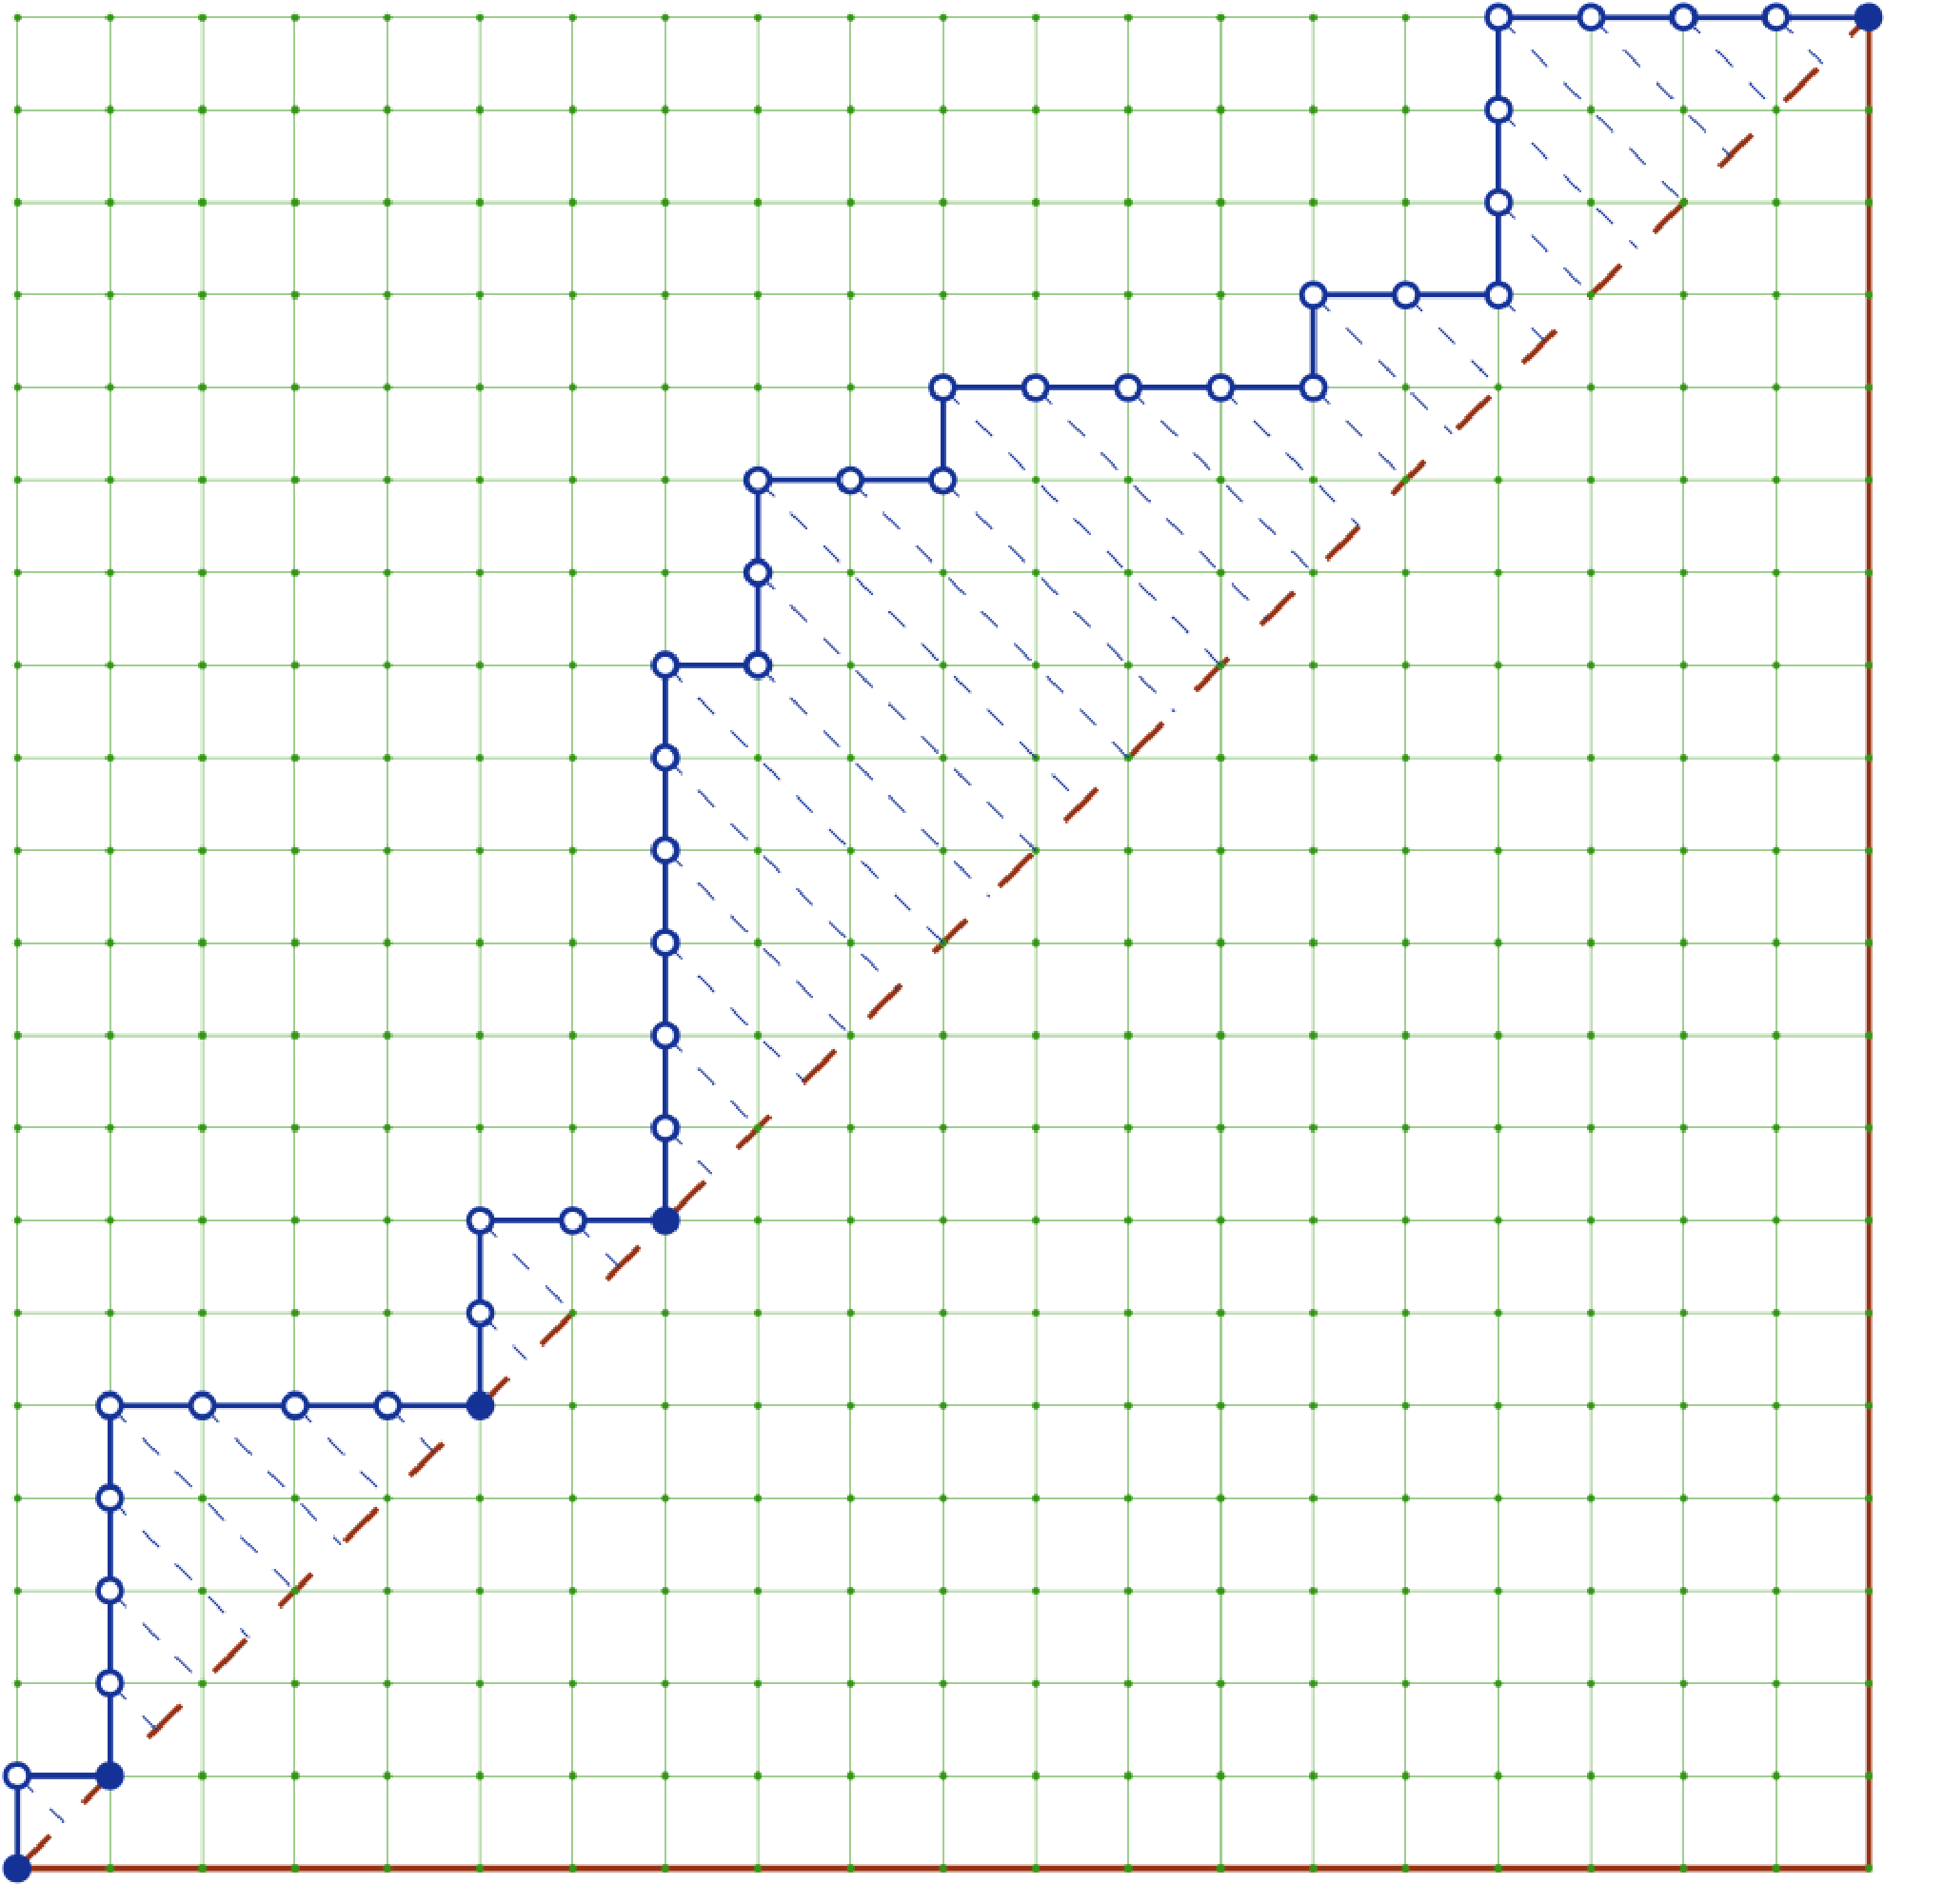
\includegraphics[width=\textwidth]{dyck/basic_dyck_path.pdf}
    \caption{Simple Dyck path with $n = 35$.}
    \label{fig:basic_dyck}
\end{figure}


\subsection{Catalan Trapezoids and Generalized Dyck Paths}
First, we define Catalan trapezoids as presented in \cite{trap}.
Let $C_k(n,m)$ be the $(n,m)^{th}$ entry of the Catalan trapezoid of order $k$,
where $C_1(n,m)$ corresponds to the Catalan triangle.

The interpretation is as follows. Consider a sequence of $n$ up-steps and $m$ down-steps,
such that the sum of any initial sub-string is not less than $1-k$.
This means that we start our Dyck path at a height of $k-1$,
and we are never allowed to cross below zero (Figure~\ref{fig:complex_dyck}).
The total number of such paths is exactly $C_k(n,m)$.
For $k = 1$, we obtain the definition of the simple Dyck path (Figure~\ref{fig:basic_dyck}).

Now, we state a result from \cite{trap} without proof
$$
C_k(n,m)=
\begin{cases}
{n+m}\choose m &0\le m<k\\
{{n+m}\choose{m}} - {{n+m}\choose{m-k}} &k\le m\le n+k-1\\
0 &m>n+k-1
\end{cases}
$$

\begin{figure}[htbp]
    \centering
    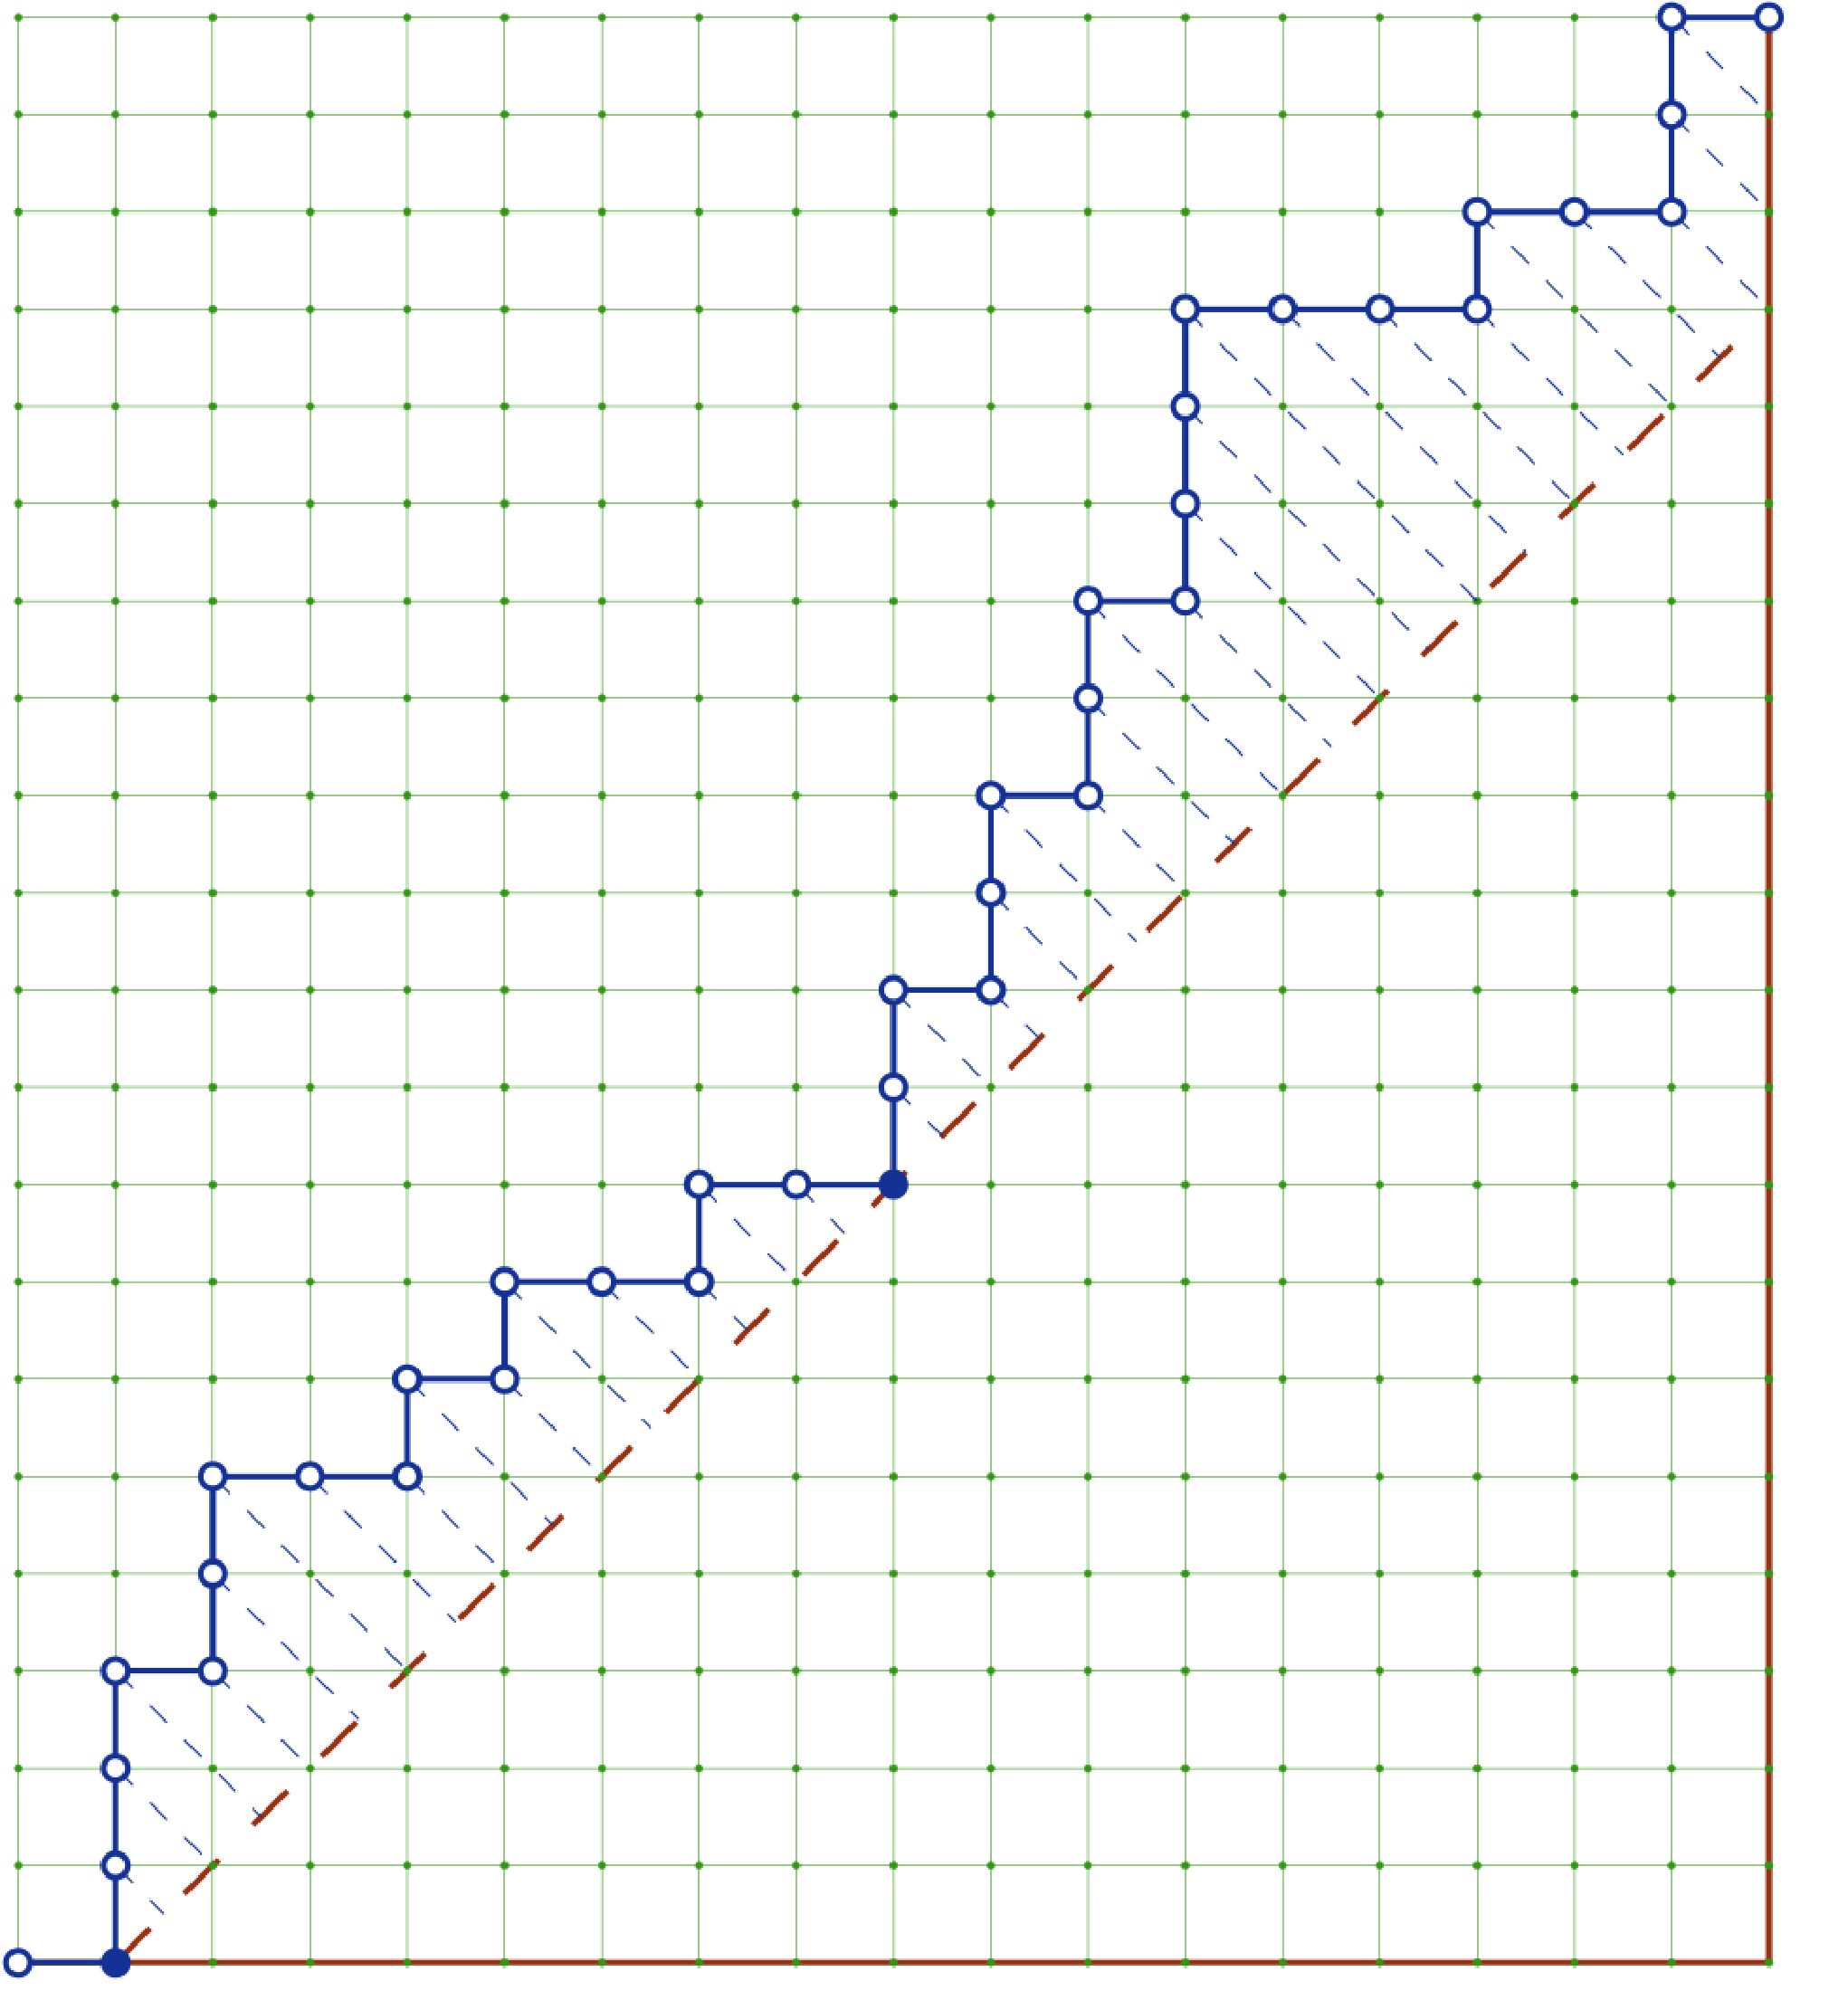
\includegraphics[width=\textwidth]{dyck/complex_dyck_path.pdf}
    \caption{Complex Dyck path with $n = 25$, $m = 22$ and $k = 3$.
             Notice that the boundary is shifted.} \label{fig:complex_dyck}
\end{figure}

\subsection{Generating Dyck Paths}
Our general recursive step is as follows.
We consider a sequence of length $2S$ comprising of $2U$ up moves ($+1$) and $2D$ down moves ($-1$).
Additionally, the sum of any initial sequence {\color{red} prefix?} canon be less than $k-1$.
Without loss of generality, let's assume that $2D\le S$. If this were not the case,
we could simply flip the sequence and negate the elements.
This essentially means that the overall Dyck path is non-decreasing.

\begin{lemma}
$S-2D = \Bo(\log n\sqrt S) \implies U-D = \Bo(\log n\sqrt S)$
\label{lem:dyck_var0}
\end{lemma}

We want to sample the height of this path after $S$ steps.
This is the same as sampling the number of $(+1)$s that get assigned to the first half of the elements in the sequence.
We define $p_d$ as the probability that exactly $D-d$ $(-1)$s get assigned to the first half.
This means that exactly $U+d$ $(+1)$s get assigned to the first half.
Consequently, the second half will contain exactly $D+d$ $(-1)$s and $U-d$ $(+1)$s.
\todo{What is $d$ is negative?}


Let us first compute this probability.
$$
p_d = \frac{D_{left}\cdot D_{right}}{D_{tot}}
$$
Here, $D_{left}$ denotes the number of valid starting sequences (first half)
and $D_{right}$ denotes the number of valid ending sequences.
Here, \textit{valid} means that each half sequence gets the appropriate number of ups and downs
and the initial sums never drop below $1-k$.
For, $D_{right}$, we will start the Dyck path from the end of the $2S$ sequence.
In this case the invalidation threshold will be a different $k'$.
This $k'$ is the final height of the $2S$ sequence. So, $k'=k+2U-2D = k+4S-2D$.
We will use this fact extensively moving forward.

Also, $D_{tot}$ is the total number of possible sequences of length $2S$, given the initial conditions.
Note that in this case the threshold remains at $k$.

\subsection{The Simple Case}
The problem of sampling reduces to the binomial sampling case when $k > \mathcal{O}(\log n)\sqrt S$ for some constant $c$.
This is because with high probability, will never dip below the threshold.
In this case, the we can simply approximate the probability as
$$
\frac{{{S}\choose{D-d}}\cdot{{S}\choose{D+d}}}{{{2S}\choose{2D}}}
$$
This is because unconstrained random walks will not dip below the $1-k$ threshold with high probability.
This problem was solved in \cite{huge} using $\mathcal O(poly(\log n))$ resources.
%Note that this uses the assumption that we have an increasing path.

\subsection{Path Segments Close to Zero}
The problem arises when we $k <\mathcal{O}(\log n)\sqrt{S}$. In this case we need to compute the actual probability,
Using the formula from \cite{trap}, we find that.
\begin{align}
D_{left} = {{S}\choose{D-d}}-{{S}\choose{D-d-k}} &&D_{right} = {{S}\choose{U-d}}-{{S}\choose{U-d-k'}}
\end{align}
Here, $k' = k+2U-2D$, and so $k' = \Bo(\log n)\sqrt S$.\todo{prove using Lemma~\ref{lem:dyck_var0}}

Finally, we compute the total number of Dyck paths as
$$
D_{tot} = {{2S}\choose{2D}}-{{2S}\choose{2D-k}}
$$

Now, we are going to use the following Lemma from \cite{huge}.
\begin{lemma}
\label{lem:huge}
Let $\{p_i\}$ and $\{q_i\}$ be distributions satisfying the following conditions
\begin{enumerate}
    \item There is a poly-time algorithm to approximate $p_i$ and $q_i$ up to $\pm n^{-2}$
    \item Generating an index $i$ according to $q_i$ is closely implementable.
    \item There exists a $poly(log n)$-time recognizable set $S$ such that
    \begin{itemize}
        \item $1-\SL{i\in S}{} p_i$ is negligible
        \item There exists a constant $c$ such that for every $i$, it holds that $p_i\le \log^{\mathcal{O}(1)} n\cdot q_i$
    \end{itemize}
\end{enumerate}
Then, generating an index $i$ according to the distribution $\{p_i\}$ is closely-implementable.
\end{lemma}

In this process, we will first disregard all values of $d$ where $|d|>\Theta(\sqrt S)$.
The probability mass associated with these values can be shown to be negligible \todo{bound variance of path}.

Next, we will construct an appropriate $\{q_i\}$ and show that $p_d < \log^{\mathcal{O}(1)} n\cdot q_d$
for all $|d|<\Theta(\sqrt S)$ and some constant $c$.
We will use the following distribution
$$
q_d = \frac{{S\choose D-d}\cdot{S\choose D+d}}{{2S\choose 2D}} = \frac{{S\choose D-d}\cdot{S\choose U-d}}{{2S\choose 2D}}
$$
It is shown in \cite{huge} that this distribution is closely implementable.

\begin{lemma}
First we show that $D_{left} \le \frac{c_1\cdot k}{\sqrt{S}}\cdot{{S}\choose{D-d}}$ for some constant $c_1$.
\end{lemma}
\begin{proof}
This involves some simple manipulations.
\begin{align}
D_{left} &= {{S}\choose{D-d}}-{{S}\choose{D-d-k}}\\
&= {{S}\choose{D-d}}\cdot \left[1-\frac{(D-d)(D-d-1)\cdots(D-d-k+1)}{(S-D-d+k)(S-D-d+k-1)\cdots(S-D-d+1)}\right]\\
&\le {{S}\choose{D-d}}\cdot \left[1-\left(\frac{D-d-k+1}{S-D+d+k}\right)^k\right]\\
&\le {{S}\choose{D-d}}\cdot \left[1-\left(\frac{U+d+k-(U-D+d+k-1)}{U+d+k}\right)^k\right]\\
&\le {{S}\choose{D-d}}\cdot \left[1-\left(\frac{U+d+k-\Bo(\sqrt{U})}{U+d+k}\right)^k\right]\\
&\le \frac{k}{\Theta(\sqrt{S})}\cdot{{S}\choose{D-d}}
\end{align}
\end{proof}

\begin{lemma}
Similarly, we show that $D_{right} < \frac{c_2\cdot k'}{\sqrt{S}}\cdot{{S}\choose{U-d}}$ for some constant $c_2$.
\end{lemma}
\begin{proof}
\begin{align}
D_{right} &= {{S}\choose{U-d}}-{{S}\choose{U-d-k'}}\\
&= {{S}\choose{U-d}}\cdot \left[1-\frac{(U-d)(U-d-1)\cdots(U-d-k'+1)}{(S-U-d+k')(S-U-d+k'-1)\cdots(S-U-d+1)}\right]\\
&\le {{S}\choose{U-d}}\cdot \left[1-\left(\frac{U-d-k'+1}{S-U+d+k'}\right)^{k'}\right]\\
&\le {{S}\choose{U-d}}\cdot \left[1-\left(\frac{2D-U-d-k+1}{2U-D+k+d}\right)^{k'}\right]\\
&\le {{S}\choose{U-d}}\cdot \left[1-\left(\frac{U+k+d - (2U-2D+2d+2k-1)}{U+k+d}\right)^{k'}\right]\\
&\le {{S}\choose{U-d}}\cdot \left[1-\left(\frac{U+k+d - \Bo(\sqrt U)}{U+k+d}\right)^{k'}\right]\\
&\le \frac{k'}{\Theta(\sqrt{S})}\cdot{{S}\choose{U-d}}
\end{align}
\end{proof}

Finally, we need to lower bound the value of $D_{tot}$.

\begin{lemma}
We claim that $D_{tot} < \frac{c_3\cdot k\cdot k'}{S}\cdot{{2S}\choose{2D}}$ for some constant $c_3$.
\end{lemma}
\begin{proof}
\begin{align}
D_{tot} &= {{2S}\choose{2D}}-{{2S}\choose{2D-k}}\\
&= {{2S}\choose{2D}}\cdot \left[1-\frac{(2D)(2D-1)\cdots(2D-k+1)}{(2S-2D+k)(2S-2D+k-1)\cdots(2S-2D+1)}\right]\\
&\ge {{2S}\choose{2D}}\cdot \left[1-\left(\frac{2D-k+1}{2S-2D+1}\right)^k\right]\\
&\ge {{2S}\choose{2D}}\cdot \left[1-\left(\frac{2U-(2U-2D+k-1)}{2U+1}\right)^k\right]\\
&\ge {{2S}\choose{2D}}\cdot \left[1-\left(\frac{(2U+1)-k'}{2U+1}\right)^k\right]\\
&\ge \frac{k\cdot k'}{\Theta(S)}\cdot{{2S}\choose{2D}}
\end{align}
\end{proof}

\begin{theorem}
We can now put these lemmas together to show that $p_d/q_d \le c = c_1\cdot c_2/c_3 = \Theta(1)$.
This satisfies all the conditions of Lemma~\ref{lem:huge} from \cite{huge}.
We simply need to set the accept probability less than $p_d/(c\cdot q_d)$.
\end{theorem}

